% Author: Miles Roberts
% last edited: 2023-03-10
% Note: this is basically just the biorxiv latex template, but with our lab logo and some small modifications to the bibliography style.
\documentclass[10pt,letterpaper]{article}
\usepackage[top=0.85in,left=0.75in,footskip=0.75in,marginparwidth=0in]{geometry}

% use Unicode characters - try changing the option if you run into troubles with special characters (e.g. umlauts)
\usepackage[utf8]{inputenc}

% clean citations
% miles: use natbib instead of whatever default is in biorxiv template
\usepackage{natbib}

% Try to add orcid ids
\usepackage[pro]{fontawesome5}

% hyperref makes references clicky. use \url{www.example.com} or \href{www.example.com}{description} to add a clicky url
\usepackage{nameref,hyperref}

% line numbers
\usepackage[right]{lineno}

% improves typesetting in LaTeX
\usepackage{microtype}
\DisableLigatures[f]{encoding = *, family = * }

% text layout - change as needed
\raggedright
\setlength{\parindent}{0.5cm}
\textwidth 7.25in 
\textheight 8.75in

% Remove % for double line spacing
%\usepackage{setspace} 
%\doublespacing

% use adjustwidth environment to exceed text width (see examples in text)
\usepackage{changepage}

% adjust caption style
\usepackage[aboveskip=1pt,labelfont=bf,labelsep=period,singlelinecheck=off]{caption}

% remove brackets from references
\makeatletter
\renewcommand{\@biblabel}[1]{\quad#1.}
\makeatother

% headrule, footrule and page numbers
\usepackage{lastpage,fancyhdr,graphicx}
\usepackage{epstopdf}
\pagestyle{myheadings}
\pagestyle{fancy}
\fancyhf{}
\rfoot{\thepage/\pageref{LastPage}}
\renewcommand{\footrule}{\hrule height 2pt \vspace{2mm}}
\fancyheadoffset[L]{2.25in}
\fancyfootoffset[L]{2.25in}

% use \textcolor{color}{text} for colored text (e.g. highlight to-do areas)
\usepackage{color}

% define custom colors (this one is for figure captions)
\definecolor{Gray}{gray}{.25}

% this is required to include graphics
\usepackage{graphicx}

% use if you want to put caption to the side of the figure - see example in text
\usepackage{sidecap}

% use for have text wrap around figures
\usepackage{wrapfig}
\usepackage[pscoord]{eso-pic}
\usepackage[fulladjust]{marginnote}
\reversemarginpar

% use xr to allow referencing figures in supplement
\usepackage{xr}
\externaldocument{supplement}

% document begins here
\begin{document}
\vspace*{0.35in}

% Add our lab logo
\begin{picture}(0,0)%
\put(375,-25){
\includegraphics[width=1.7129in]{Josephs_transparent.png}}%
\end{picture}

% title goes here:
\begin{flushleft}
{\Large
\textbf\newline{Josephs Lab Manuscript Template (title goes here)}
}
\newline
% authors go here:
\\
\href{https://orcid.org/0000-0001-9854-701X}{\faGraduationCap}Author 1\textsuperscript{1*},
\href{https://orcid.org/0000-0001-9854-701X}{\faGraduationCap}Author 2\textsuperscript{2,3},
\href{https://orcid.org/0000-0001-9854-701X}{\faGraduationCap}Author 3\textsuperscript{3}
\\
\bigskip
\bf{1} Affiliation 1
\\
\bf{2} Affiliation 2
\\
\bf{3} Affiliation 3
\\
\bigskip
* corresponding@author.com

\end{flushleft}

% now start line numbers
\linenumbers

\section*{Abstract}

making changes 

% the * after section prevents numbering
\section*{Introduction}

yay yay yay

To add a parenthetical citation, use \citep{corbett-detig_natural_2015}. To add an in-text citation, use \citet{corbett-detig_natural_2015}. To add an alternative citation, use \citealt{corbett-detig_natural_2015}. To include all authors in the citation, use \citet*{corbett-detig_natural_2015} or \citep*{corbett-detig_natural_2015} or \citealt*{corbett-detig_natural_2015}.

To add hyperlinks, use: \href{https://www.overleaf.com/learn}{Example hyperlink}


\section*{Materials and Methods}

\subsection*{Section 1}

Separate your methods into subsections

\subsection*{Section 2}

\subsubsection*{Section 2.1}

Add sub-sub-sections for especially detailed procedures

\subsubsection*{Section 2.2}

Example of an equation

\begin{equation}
\pi_i = \left( \frac{n_i}{n_i-1} \right) \left( 1 - \sum_{j = 1}^{2} p_{ij}^2 \right)
\label{eq:pi}
\end{equation}

You can reference the equation as so (See equation \ref{eq:pi})

\section*{Results}

% Add figures like so:
% Figure tutorial: https://www.overleaf.com/learn/latex/Inserting_Images
\begin{figure}[!h]
\centering
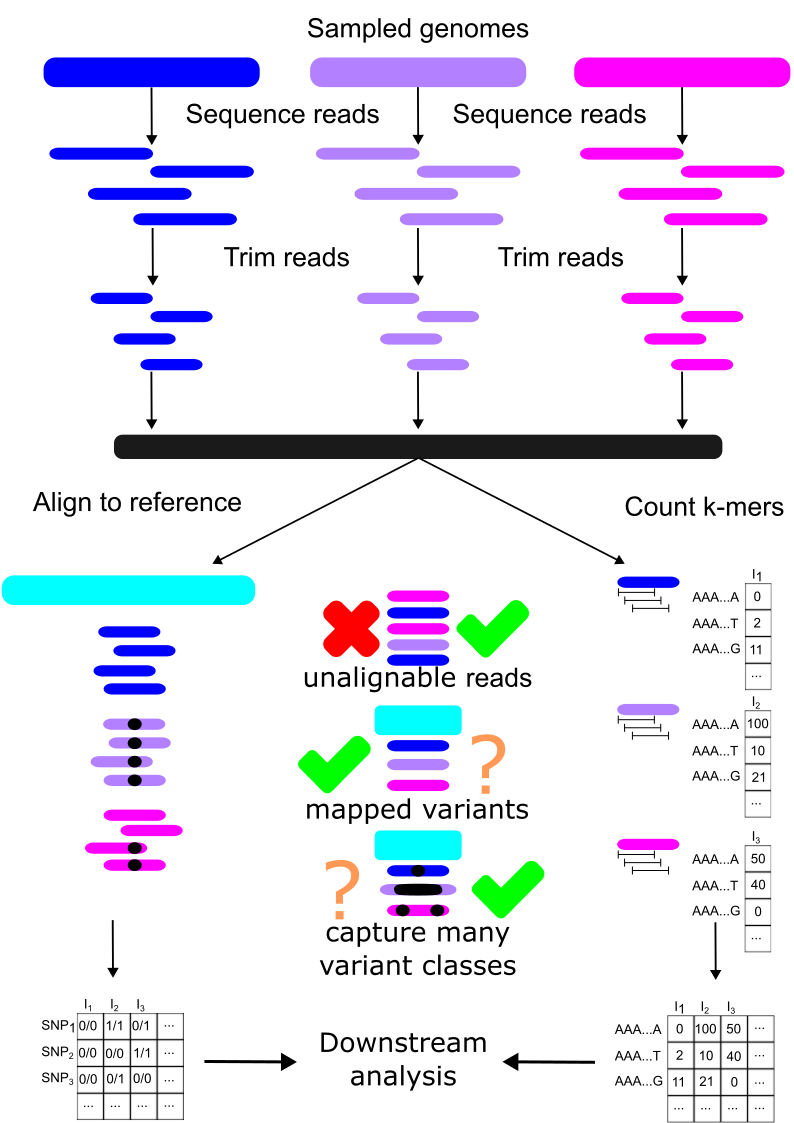
\includegraphics[width=0.8\linewidth]{figures/main/a_main_figure.png}
\caption{Add a caption to describe your figure, then also add a label so that you can reference the figure in the text}%
\label{fig:logo}
\end{figure}

Type your results here. Reference your figures like so (see Figure \ref{fig:logo}).

foo bar foo bar lol lol lol
like so: Figure \ref{fig:sup}.

\section*{Discussion}

Tracking changes

Discuss your results here

\section*{Data availability}

Add links to your github repo and data repository. List what pieces of data are contained in each supplementary file.

\section*{Acknowledgments}

Thank informal reviewers and peer reviewers

\section*{Author contributions}

Author 1 did all of the work. Author 2 and 3 provided emotional support.

\section*{Funding}

List the grants (and their associated identifiers) that funded you during the period you conceived of or performed this research

\section*{Conflicts of interest}

Say ``none declared" or explain potential conflicts

% Stop line numbers
\nolinenumbers

%This is where your bibliography is generated. Make sure that your .bib file is actually called library.bib
% Most citation managers have options to directly export .bib files
\bibliography{library}

%This defines the bibliographies style. Search online for a list of available styles.
\bibliographystyle{apalike}
\setcitestyle{authoryear, open={(},close={)}}

\end{document}

